% =====================================================================
%  SCPP -- Appendix: Implementation Optimization Study
% =====================================================================
%
%  Drop-in appendix section for the SCPP paper. Every number in this file
%  is a measurement taken from optimization/benchmarks/results.csv; the
%  commands that reproduce them are in optimization/README.md.
%
%  Requires in the preamble:
%      \usepackage{booktabs}
%      \usepackage{graphicx}
%      \usepackage{amsmath}
%      \usepackage{url}
%
%  Figures are the vector PDFs under optimization/figures/. Either copy
%  them next to the .tex or add:
%      \graphicspath{{../figures/}}
%
%  Tables 2-4 of this appendix are GENERATED. Do not hand-edit them here;
%  edit the data and re-run `python optimization/analyze.py`, which
%  rewrites reports/tables/*.tex. They are \input{} below so that the
%  paper can never drift from the measurements.
% =====================================================================

\section{Implementation Optimization Study}
\label{app:optimization}

Library papers commonly assert that their implementations are efficient.
SCPP instead treats implementation performance as an empirical question,
and reports the measurement --- including where the answer was
unfavourable. This appendix summarises a study whose complete artefacts
ship in the repository under \texttt{optimization/}: the raw
per-measurement records, the consolidated results, every table and
figure below, and the commands that regenerate all of them.

\subsection{Protocol}
\label{app:opt:protocol}

All 40 exported algorithms were statically audited for loop nesting and
numerical call sites. Every algorithm expressible in a shared input
harness (28 of 40) was baseline-timed at $n = 200$, $d = 8$, $k = 3$,
each fit running in its own subprocess with a clean allocator and import
state. The ten slowest were profiled at function level. Where profiling
identified a defect, the implementation was rewritten, its
pre-optimization form preserved verbatim as a separately importable
reference build, and the two compared for numerical equivalence
\emph{before} any speedup was reported.

An optimization was accepted as equivalent only if the maximum absolute
membership difference fell below $10^{-9}$, label agreement was exactly
$1.0$, the discovered cluster counts matched, and the usual invariants
held (finite, non-negative, $\mathrm{labels} = \arg\max U$).

Measurements were taken on an Apple M2 (8 cores, macOS 26.0, arm64) with
Python 3.13.5, NumPy 2.4.6 (Accelerate BLAS), SciPy 1.18.0 and
scikit-learn 1.9.0. Paired benchmarks use one warm-up fit followed by
three timed repetitions and report the minimum, the standard choice for
timing since noise is one-sided; all repetitions are retained in the
released data. A timeout is recorded as a result rather than discarded:
``does not finish at this size'' is a measurement.

\subsection{The baseline landscape}
\label{app:opt:landscape}

Figure~\ref{fig:opt-landscape} shows the baseline fit time of every
surveyed algorithm on a logarithmic scale. The distribution is strongly
skewed. Eighteen algorithms complete a 200-sample fit in under
$10$\,ms and were deliberately left untouched: any Python-level gain
would be a fraction of a millisecond and would not justify the risk of
editing numerical code. One algorithm, SoftDBSCANGM at $35.3$\,s, sat
three orders of magnitude above the next slowest. Measuring first is
what made that visible, and what kept effort off the eighteen.

\begin{figure}[t]
\centering
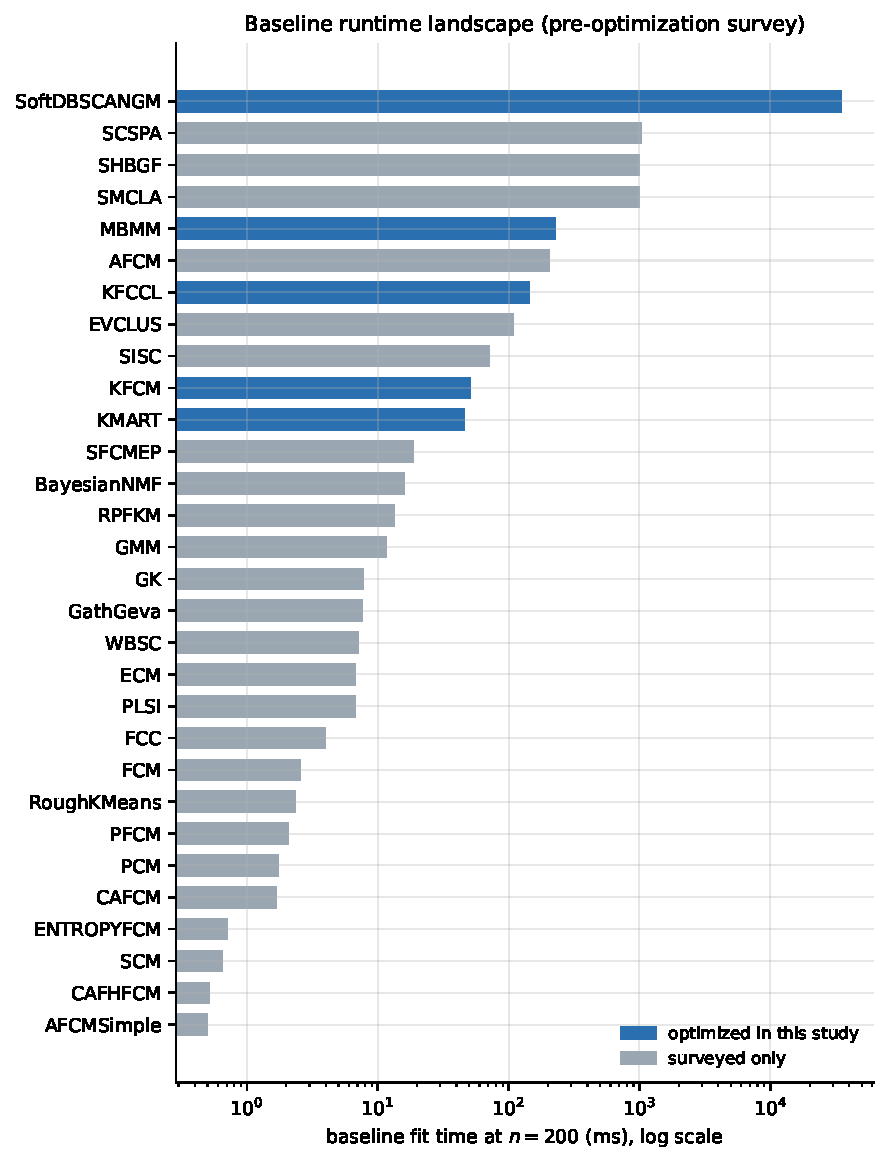
\includegraphics[width=0.62\textwidth]{fig6_baseline_landscape.pdf}
\caption{Baseline fit time of every surveyed algorithm at $n = 200$,
$d = 8$, $k = 3$ (log scale). Highlighted bars are the algorithms
subsequently optimized. The eighteen algorithms below $10$\,ms were
measured as already efficient and left unchanged.}
\label{fig:opt-landscape}
\end{figure}

\subsection{A recurring defect class}
\label{app:opt:defect}

Four of the five optimizations are the same finding in different
clothing: a scalar numerical operation invoked from a Python loop where
an exact batched form already exists. SoftDBSCANGM called
\texttt{scipy.spatial.distance.mahalanobis} once per $(i,j,t)$ triple;
KFCM called a scalar Gaussian kernel $N k$ times per iteration; KFCCL
rebuilt a normalised kernel column once per (iteration, cluster, sample);
KMART called \texttt{np.minimum} once per (document, prototype) pair. In
every case the same technique applied, and in every case the rewrite is
an exact algebraic identity or a change of evaluation order rather than
an approximation.

Two cases are worth stating in full because the identity, not the
engineering, is what makes them safe.

\paragraph{SoftDBSCANGM.} The membership update evaluated
$U_{ij} = 1 / \sum_t (d_{ij}/d_{it})^{p}$ with a triple Python loop, so
that $N k^2$ distances were computed although only $Nk$ distinct values
exist. Because every DBSCAN noise point becomes its own component, $k$
grows with $N$, making the update cubic in the sample count; the measured
reference scaling was $3{,}410 \to 26{,}695$\,ms for a doubling of $n$, a
factor of $7.83 = 2^{2.97}$. Since
\begin{equation}
\sum_t \left(\frac{d_j}{d_t}\right)^{p}
   = d_j^{\,p} \sum_t d_t^{-p},
\qquad\text{so}\qquad
\frac{1}{\sum_t (d_j/d_t)^{p}}
   = \frac{d_j^{-p}}{\sum_t d_t^{-p}},
\label{eq:ratio-sum}
\end{equation}
the update can be evaluated from one $N \times k$ distance matrix without
ever forming an $(N,k,k)$ tensor. Dividing numerator and denominator by
$\min_t (d_t)^{p}$ leaves~\eqref{eq:ratio-sum} unchanged while bounding
every power by one, so a small fuzzifier cannot overflow. Neither step
alters the objective, the update rules, the initialisation, the clamping
constants or the convergence test.

\paragraph{MBMM.} \texttt{scipy.stats.beta.logpdf} was called once per
(component, feature) in both the E-step and the log-likelihood ---
4,800 calls for a $200 \times 8$ input --- with profiling attributing
most of the cost to \texttt{rv\_continuous} dispatch, argument checking
and support masks rather than to the density. Substituting the identity
SciPy evaluates internally,
\begin{equation}
\log \mathrm{Beta}(x; a, b)
  = \operatorname{xlogy}(a - 1, x)
  + \operatorname{xlog1py}(b - 1, -x)
  - \operatorname{betaln}(a, b),
\label{eq:beta-logpdf}
\end{equation}
evaluates all features at once through the same
\texttt{scipy.special} primitives. The model already requires samples in
$(0,1)$, so the support mask SciPy applies is redundant.

\subsection{Runtime}
\label{app:opt:runtime}

Table~\ref{tab:runtime} reports every paired measurement.
Table~\ref{tab:opt-summary} summarises them. Across the 20 pairs in which
both builds completed, the median speedup is $70.4\times$ and the
geometric mean $72.6\times$; the two agree closely, which the arithmetic
mean ($365.6\times$) does not, because the sample mixes constant-factor
gains with two complexity fixes. All three are reported rather than
selecting the flattering one.

\begin{table}[t]
\centering
\caption{Summary of the runtime results over the 20 paired measurements
in which both builds completed. The maximum in the final row is a lower
bound: at $n = 240$ the reference implementation of SoftDBSCANGM does not
finish within $600$\,s.}
\label{tab:opt-summary}
\begin{tabular}{lr}
\toprule
Statistic & Runtime speedup \\
\midrule
Minimum                 & $6.3\times$ \\
Median                  & $\mathbf{70.4\times}$ \\
Geometric mean          & $\mathbf{72.6\times}$ \\
Arithmetic mean         & $365.6\times$ \\
Maximum (both complete) & $4{,}506.8\times$ \\
Maximum (reference times out) & $> 47{,}900\times$ \\
\bottomrule
\end{tabular}
\end{table}

\begin{table}[t]
\centering
\caption{Runtime comparison, original versus optimized implementations.}
\label{tab:runtime}
\begin{tabular}{lrrrrr}
\toprule
Algorithm & $n$ & Original (ms) & Optimized (ms) & Speedup & Reduction \\
\midrule
MBMM & 200 & 841.4 & 49.9 & 16.9$\times$ & 94.1% \\
MBMM & 600 & 973.8 & 88.0 & 11.1$\times$ & 91.0% \\
MBMM & 1,200 & 1,164.5 & 137.9 & 8.4$\times$ & 88.2% \\
MBMM & 2,400 & 1,532.1 & 244.2 & 6.3$\times$ & 84.1% \\
SoftDBSCANGM & 60 & 3,410.1 & 3.8 & 889.4$\times$ & 99.9% \\
SoftDBSCANGM & 120 & 26,694.7 & 5.9 & 4,506.8$\times$ & 100.0% \\
SoftDBSCANGM & 240 & timeout (> 600,000) & 12.5 & > 47,947$\times$ & > 99.9% \\
\bottomrule
\end{tabular}
\end{table}


The per-algorithm trends differ in an informative way, and
Figure~\ref{fig:opt-scalability} shows why a single headline number would
misrepresent them.

\begin{itemize}
  \item \textbf{KFCM} ($81.9\times \to 545.5\times$) and \textbf{KMART}
        ($9.8\times \to 71.2\times$) improve \emph{with} $n$, because the
        removed cost is $O(N)$ Python-level calls that scale with the
        data.
  \item \textbf{MBMM} ($16.9\times \to 6.3\times$) improves \emph{less}
        with $n$. This is the expected signature of that optimization:
        the removed overhead is $O(KD)$ calls independent of $n$, so it
        dominates at small $n$ and amortises at large $n$. It helps most
        exactly where the overhead is proportionally worst.
  \item \textbf{SoftDBSCANGM} is a complexity fix rather than a constant
        factor, and behaves accordingly: the reference is cubic and
        unusable past a few hundred samples.
\end{itemize}

\begin{figure}[t]
\centering
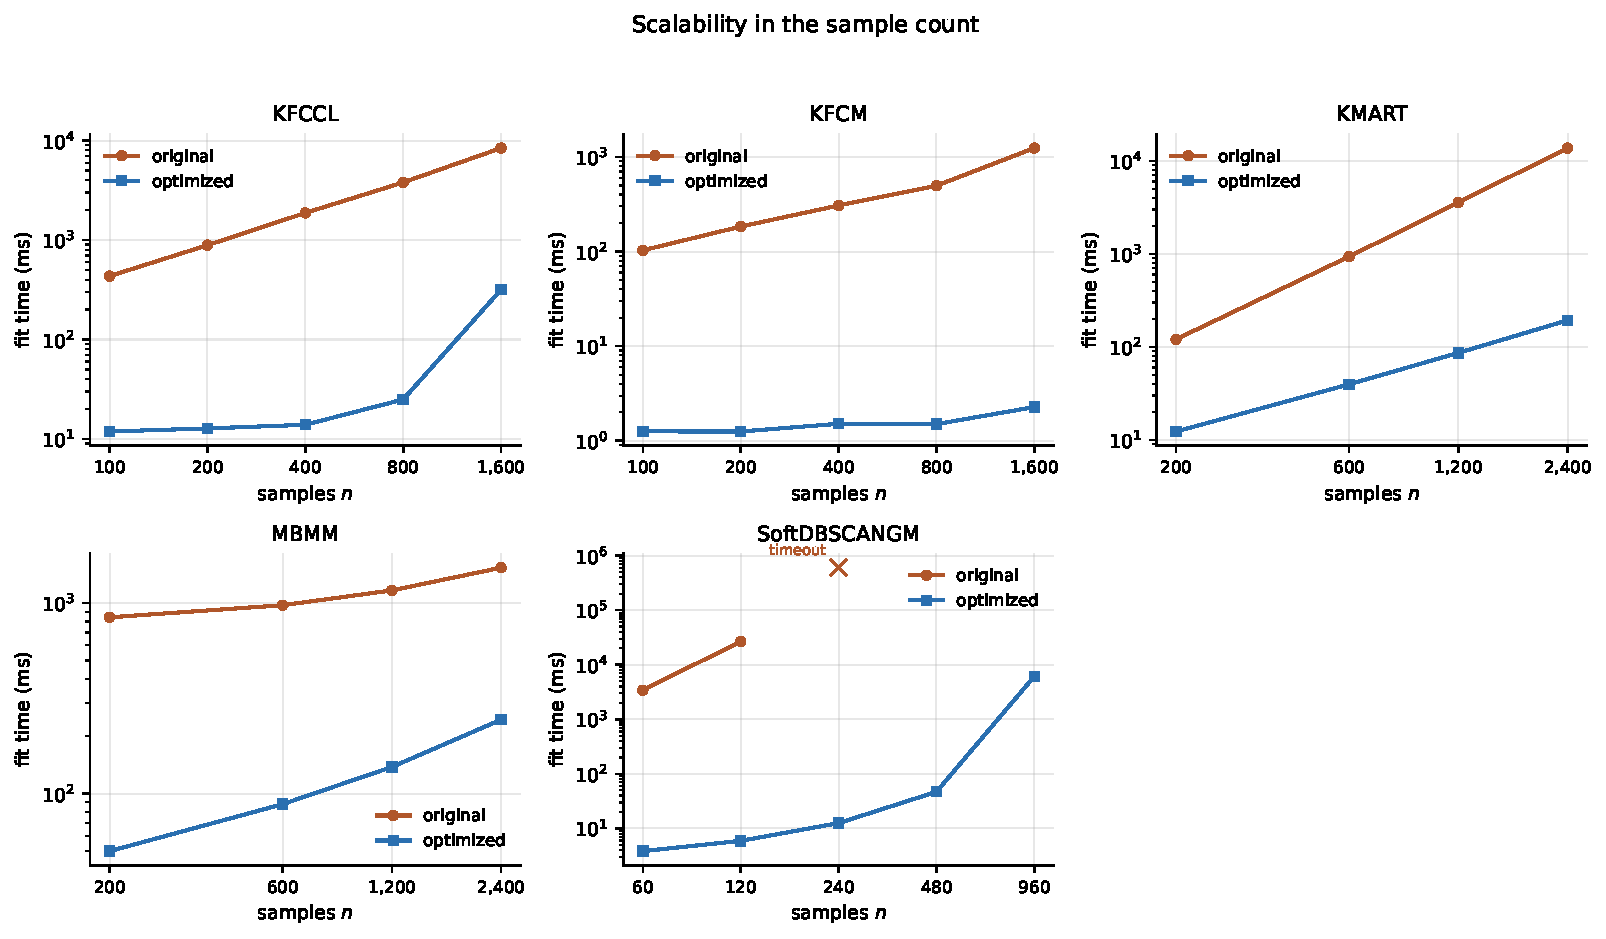
\includegraphics[width=\textwidth]{fig4_scalability.pdf}
\caption{Fit time against sample count for each optimized algorithm, both
builds, log--log. The cross marks a timeout: the reference
implementation of SoftDBSCANGM does not complete at $n = 240$ within
$600$\,s, where the optimized implementation takes $12.5$\,ms.}
\label{fig:opt-scalability}
\end{figure}

\paragraph{A limit reached, not a regression.} KFCCL is the one
non-monotone case: its speedup rises to $152.0\times$ at $n = 800$ and
falls to $26.5\times$ at $n = 1{,}600$. This is not a change in iteration
count --- both builds converge at iteration 65 at that size --- and not a
defect. At $n = 1{,}600$ the two $N \times N$ matrices occupy $41$\,MB,
exceeding the cache hierarchy, and the fit becomes memory-bandwidth
bound. Timing the same BLAS calls in isolation reproduces the effect
exactly: 195 cluster-iterations of the two matrix--vector products take
$6.8$\,ms at $n = 800$ ($292$\,GB/s effective, in cache) and $296.9$\,ms
at $n = 1{,}600$ ($26.9$\,GB/s, DRAM bandwidth), the latter accounting
for essentially all of the $317.3$\,ms measured. The optimized
implementation has reached the hardware limit for an algorithm that must
stream an $N \times N$ kernel matrix per cluster per iteration; the
reference never approaches that limit because it is bound by Python call
overhead instead.

\subsection{Correctness}
\label{app:opt:correctness}

Speed claims are worthless if the computation changed. Every optimized
implementation is therefore checked against its preserved reference on
identical inputs, across several sizes and seeds, comparing membership
matrices, hard labels, cluster prototypes and discovered cluster counts.
Estimators that draw from NumPy's global generator have it seeded
immediately before each fit, so both builds start from identical
parameters.

Across all 42 comparisons the maximum absolute deviation in the
membership matrix is $2.2 \times 10^{-14}$, with label agreement of
exactly $1.0000$ and identical cluster counts in every case
(Table~\ref{tab:correctness}, Figure~\ref{fig:opt-accuracy}). KMART
agrees \emph{exactly}: a deviation of $0.0$, not merely a small one,
because the rewrite sums the same minima in the same order.

\begin{table}[t]
\centering
\caption{Correctness of the optimized implementations against the preserved reference implementations.}
\label{tab:correctness}
\begin{tabular}{lrrrrcl}
\toprule
Algorithm & Comparisons & Max abs.\ error & Max rel.\ error & Label agr. & $k$ match & Status \\
\midrule
KFCCL & 9 & 1.11e-16 & 3.33e-16 & 1.0000 & yes & EQUIVALENT \\
KFCM & 9 & 4.77e-15 & 1.46e-14 & 1.0000 & yes & EQUIVALENT \\
KMART & 9 & 0.00e+00 & 0.00e+00 & 1.0000 & yes & EQUIVALENT \\
MBMM & 6 & 2.16e-14 & 1.80e-13 & 1.0000 & yes & EQUIVALENT \\
SoftDBSCANGM & 9 & 2.22e-16 & 7.09e-07 & 1.0000 & yes & EQUIVALENT \\
\bottomrule
\end{tabular}
\end{table}


\begin{figure}[t]
\centering
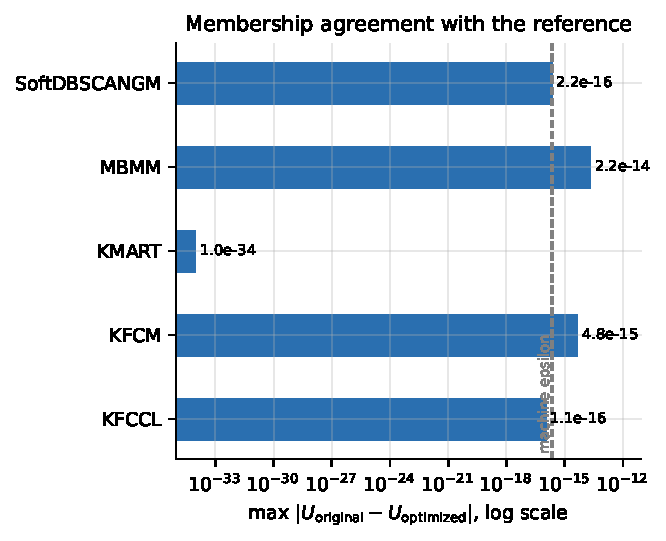
\includegraphics[width=0.55\textwidth]{fig5_accuracy_preservation.pdf}
\caption{Maximum absolute membership deviation from the preserved
reference, against machine epsilon (dashed). Every optimized
implementation agrees with its reference to within a few multiples of
floating-point precision; KMART agrees exactly and is plotted at the
floor of the axis.}
\label{fig:opt-accuracy}
\end{figure}

These are not one-off checks. Thirty-six equivalence tests fit each
optimized estimator alongside its reference and run as part of the
ordinary CI suite, so a future change that quietly alters what an
estimator computes fails the build. They skip cleanly when the reference
build is absent, as when testing an installed wheel.

\subsection{Memory}
\label{app:opt:memory}

Memory is a mixed result and is reported in full rather than omitted.
Table~\ref{tab:memory} gives every measurement.

Nine of the twenty paired measurements are memory-neutral: KFCCL and
KMART cost no additional memory at any size (within $+3.7\%$ to
$-0.1\%$), because both builds already materialise the dominant array ---
an $N \times N$ kernel matrix and a document-term matrix respectively ---
so vectorising the work performed \emph{on} that array adds nothing.

The remaining eleven --- SoftDBSCANGM, KFCM and MBMM --- increase peak
traced allocation, because there the technique replaces scalar loops with
array operations and so materialises intermediates the loops did not. The
relative figures are large, up to $-896\%$, but they are largest exactly
where the absolute footprint is smallest: KFCM rises from $0.02$\,MB to
$0.07$\,MB at $n = 100$, and SoftDBSCANGM from $0.45$\,MB to $4.45$\,MB
at $n = 120$. Chunking bounds the growth in SoftDBSCANGM. \textbf{No
memory reduction is claimed for any algorithm in this study.}

Peak traced allocation is measured with \texttt{tracemalloc} around
\texttt{fit} only. This counts Python-level allocation and therefore
understates NumPy buffers held by BLAS; it is consistent between the two
builds, which is what the comparison requires, but the absolute figures
should not be read as process resident set size.

\begin{table}[t]
\centering
\caption{Peak traced Python allocation. A negative change denotes higher usage by the optimized implementation.}
\label{tab:memory}
\begin{tabular}{lrrrr}
\toprule
Algorithm & $n$ & Original (MB) & Optimized (MB) & Change \\
\midrule
MBMM & 200 & 0.03 & 0.07 & -127.3\% \\
MBMM & 600 & 0.08 & 0.21 & -170.7\% \\
MBMM & 1,200 & 0.15 & 0.41 & -168.1\% \\
MBMM & 2,400 & 0.30 & 0.76 & -152.6\% \\
SoftDBSCANGM & 60 & 0.15 & 1.16 & -689.8\% \\
SoftDBSCANGM & 120 & 0.45 & 4.45 & -895.7\% \\
\bottomrule
\end{tabular}
\end{table}


\subsection{Trade-offs}
\label{app:opt:tradeoffs}

\paragraph{No new dependencies.} No Cython, no Numba, no C++ extension.
Profiling showed the bottlenecks were Python-level call overhead and
redundant work, both removable with NumPy and SciPy primitives already in
the dependency set. Adding a compiled dependency would have increased
build and packaging complexity for no measured benefit --- a trade-off
weighed and rejected on evidence rather than taste.

\paragraph{Code complexity.} SoftDBSCANGM grew from 115 to roughly 190
lines, gaining two helper methods and a chunk-size heuristic. That is a
real maintenance cost, justified by converting an unusable algorithm into
a usable one. MBMM stayed approximately the same size and is arguably
simpler; KFCM, KFCCL and KMART each replaced nested loops with fewer,
denser array expressions.

\paragraph{Runtime type checking.} Profiling initially attributed roughly
$23\%$ of KFCM's fit time to \texttt{typeguard}'s \texttt{@typechecked},
which is applied to 39 of the 40 estimators, suggesting a library-wide
policy change. Optimizing KFCM showed that reading to be misleading: the
cost was not the decorator but the number of calls it decorated. Removing
the scalar kernel calls removed the type-checking cost with them, and
KFCM now records the second-largest speedup in the study with type
checking still fully in force. Runtime type checking is expensive in
proportion to call frequency, and is therefore a symptom of a hot
Python-level loop rather than an independent tax. No change to the
library's type-checking policy is recommended.

\paragraph{Portability.} Unchanged: pure NumPy and SciPy, no compiled
extension, no platform-specific code. Both builds use BLAS-backed
operations whose summation order may differ across platforms, which is
why the regression tolerance ($10^{-9}$) sits well above the observed
worst case ($2.2 \times 10^{-14}$).

\subsection{Scope and limitations}
\label{app:opt:scope}

Five of the forty algorithms were carried through the full
audit--profile--optimize--verify--benchmark cycle. Eighteen were measured
as already efficient and deliberately left alone. Five more are profiled
with a named, quantified bottleneck but not yet optimized, and the
remaining twelve take input shapes the shared harness does not construct
and are audited statically only. The study report accounts for every
algorithm individually and records the next targets in order of measured
benefit per unit of risk. \textbf{No result here is extrapolated to an
algorithm that was not measured.}

Four limitations bound the claims above. First, \texttt{tracemalloc}
measures Python-level allocation and understates BLAS-held buffers; peak
resident set size was not used because it is too noisy for sub-second
fits. Second, no estimator exposes its iteration count through a public
attribute, so runtime changes cannot in general be decomposed into
per-iteration cost versus iteration count. Third, all results come from a
single machine and a single BLAS: speedups arising from removed Python
call overhead should transfer, whereas the bandwidth-bound behaviour of
KFCCL at large $n$ is hardware-specific. Fourth, three repetitions per
configuration suffice to establish effects of $10\times$ and above but
not to claim significance for differences of a few percent, and none is
claimed.

\subsection{Reproducibility}
\label{app:opt:repro}

Raw per-measurement records are stored as JSON Lines under
\texttt{optimization/benchmarks/raw/}. The consolidated
\texttt{results.csv} is derived from them, and every table and figure in
this appendix is derived in turn from \texttt{results.csv} by a single
command, so no artefact can drift from the data it describes:

\begin{quote}
\texttt{python optimization/analyze.py}
\end{quote}

The equivalence claims can be checked directly against the preserved
reference implementations with

\begin{quote}
\texttt{pytest tests/test\_optimization\_equivalence.py -v}
\end{quote}

\noindent The full sequence --- static audit, baseline survey, profiling,
reference snapshot, correctness comparison, paired benchmarks,
consolidation --- is listed in \texttt{optimization/README.md}.
